\chapter{Analyse}

\section{Domäne}

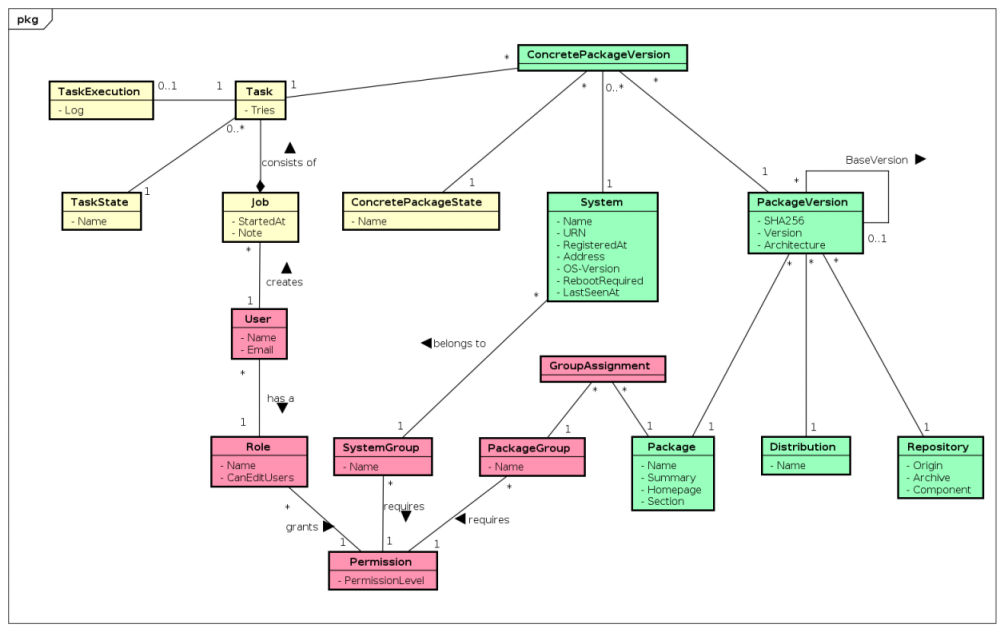
\includegraphics[width=\textwidth]{files/DomainModel_small}

\subsection{Erläuterungen}

\subsubsection{System}

Ein System repräsentiert einen einzelnen Server, auf welchem die Updates verwaltet werden sollen. Relevante Daten über die Systeme werden erfasst respektive beim Registrieren durch den Agent mitgeteilt.

\subsubsection{Package}

Ein Package ist ein einzelnes Applikationspaket, welches vom Paketmanager (hier apt) verwaltet wird. Beispiele dafür sind vim, openssl oder sudo. Das Paket selbst ist unabhängig von Versionen oder Distributionen.

\subsubsection{PackageVersion}

Eine Paket-Version ist eine verfügbare Version eines bestimmten Paketes auf einem spezifischen Repository/einer Distribution.

\subsubsection{ConcretePackageVersion}

Eine Paket-Version kann mit einem System in Verbindung gebracht werden, zum Beispiel indem der Agent eine bestimmte Paket-Version als ausstehendes Update meldet. Diese Verbindung ist eine konkrete Paket-Version und zeigt, welchen Zustand diese Version auf diesem Paket hat: Installiert, veraltet, ausstehend, fehlgeschlagen oder in Auftrag gegeben.

\subsubsection{Distribution}

Eine Distribution, oft auch "Distro" genannt, ist ein Betriebssystem basierend auf dem Linux-Kernel. Beispiele: Debian, Suse oder Ubuntu. Diese werden wiederum in spezifische Distros unterteilt, etwa bei Ubuntu auf Ubuntu 12.04 precise, 14.04 trusty oder 16.04 xenial. 

\subsubsection{Job}

Ein Job wird dann erstellt, wenn ein Benutzer einen Auftrag erteilt. Pro betroffenem System enthält dieser Job einen Task, welcher dann an die Agenten geschickt wird.

\subsubsection{Task}

Ein Task enthält alle konkreten Aufträge für ein spezifisches System, welche von einem User in einem Durchgang erfasst wurden. Ein Task kann sich in den folgenden Zuständen befinden:

\begin{itemize}
    \item Erledigt 
    \item Fehlgeschlagen 
    \item Ausstehend
    \item In Bearbeitung
    \item Nicht zugestellt
\end{itemize}

\section{Konkurrenz} \label{sec:analysis:competition}

Hier werden bereits existierende Lösungen für ähnliche Problemstellungen vorgestellt und analysiert sowie mit der Lösung \gls{upd89} verglichen.

\newcommand{\competitor}[8]{
	\begin{tabularx}{\linewidth}{lX}
		\toprule
		\textbf{Produkt} & #1\\
		\midrule
		\textbf{Hersteller} & #2\\
		\textbf{Beschreibung} & #3\\
		\textbf{Features} & #4\\
        \textbf{Lizenz} & #5\\
		\textbf{Kosten} & #6\\
        \textbf{URL} & #7\\
        \textbf{Eignung} & #8\\
		\bottomrule
	\end{tabularx}
}

\subsection{Landscape}

\competitor{Landscape}
{Canonical}
{Landscape von Canonical ist ein proprietärer Web-Service für das Managen von Ubuntu-Systemen an einem zentralen Ort.

Es kann Software verwaltet und installiert werden, ebenso Security-Updates. Updates können auch automatisch installiert oder wieder entfernt werden.

Landscape unterstützt neben Servern auch Desktops.}
{
- Deployment

- Software und Update Management inkl. Repository-Verwaltung

- Monitoring, inkl. Prozess-Zugriff sowie div. Hardware-Abfragen

- RBAC (Role-Based Access Control)
}
{Proprietär}
{Kostenlos, benötigt aber eine Advantage-Lizenz. Diese kostet im Minimum 320 USD pro Server pro Jahr.\footnote{Quelle: \purl{http://www.ubuntu.com/management/ubuntu-advantage}}}
{\purl{https://landscape.canonical.com/}}
{Abgesehen von den hohen Kosten ist Landscape nicht Open-Source. Die Lösung ist auch zu umfangreich und bietet viele Funktionen, welche bei Nine bereits durch andere Tools abgedeckt werden (z.B. Deployment, Monitoring).}

\subsection{Ansible}

\competitor{Ansible}
{AnsibleWorks, Inc.}
{Ansible ist eine Plattform zur Automatisierung von Tasks und zur Orchestrierung. Sie kombiniert Softwareverteilung, Kommando-Ausführung und Konfigurationsmanagement.Server werden via SSH angesprochen, es ist kein Agent erforderlich.

Ansible Tower die zentrale Web-basierte Kommandozentrale und ist Open-Source.\footnote{Quelle: \purl{https://www.ansible.com/subscription-agreement}}}
{
- Applikations-Deployment

- Konfigurations-Management

- User-definierbare Playbooks für Tasks

- REST-Schnittstelle für Einbinden in andere Systeme
}
{GNU General Public License v3}
{Im Enterprise-Paket kostet Ansible Tower 50 USD pro Server pro Jahr für > 1000 Server.\footnote{Quelle: \purl{https://www.ansible.com/pricing}}}
{\purl{https://www.ansible.com/}}
{Hier beläuft sich der totale Preis bei 1500 Systemen auf 75'000 USD pro Jahr, nur um die Updates zu verwalten. Ansible, vor allem auch mit Ansible-Galaxy kombiniert, bietet viel mehr Funktionalität, als Nine benötigt.}

\subsection{Spacewalk}

\competitor{Spacewalk}
{Red Hat}
{Spacewalk ist eine Open-Source Systemmanagement-Lösung für Linux-Systeme. Es basiert auf einer Community, von welcher auch der Support kommt.

Es bietet unter anderem auch ein Update-Management über Systeme und Systemgruppen hinweg. Das Ganze funktioniert über eine zentrale Web-Applikation.

Spacewalk unterstützt Fedora, CentOS, SLE und Debian.}
{
- Inventar über Hardware und installierte Software

- Installation von Software und Updates

- Konfigurationen verteilen und managen

- Content-Verteilung
}
{GNU General Public License v2}
{Kostenlos\footnote{Quelle: \purl{http://spacewalk.redhat.com/faq.html}}}
{\purl{http://spacewalk.redhat.com/}}
{``Support für Debian/Ubuntu experimentell, Eierlegende Wollmillchsau''\footnote{Quelle: interne Evaluation von Nine.ch}}

\subsection{WSUS}

\competitor{Windows Server Update Services}
{Microsoft}
{Windows Server Update Services ist eine proprietäre Update-Software von Microsoft für zentralisiertes Managen von Patches für Microsoft-Server.}
{
- Verteilen der Updates, einmaliges Herunterladen

- Client-Komponente, welche mit dem Manager kommuniziert und Status-Details liefert

- Gruppieren von Systemen
}
{Proprietär}
{Kostenlos\footnote{Quelle: \purl{https://technet.microsoft.com/en-us/windowsserver/bb332157}}}
{\purl{https://technet.microsoft.com/de-de/windowsserver/bb332157.aspx}}
{WSUS eignet sich nur für Microsoft-Produkte. Da Nine.ch ausschliesslich Linux-basierende Server verwendet, fällt WSUS aus technologischen Gründen weg.}

\subsection{Puppet}

\competitor{Puppet}
{Puppet Labs}
{Puppet ist ein Tool um Systeme zu konfigurieren, Software zu installieren oder Programme auszuführen sowie um Daten zu synchronisieren.

Puppet ist als Open-Source oder als kostenpflichtige Enterprise-Version erhältlich. }
{
- Unterstützt verschiedene Linux- und Windows-Systeme

- in Ruby geschrieben

- deklarative Sprache zur Ressourcenbeschreibung für Systemkonfigurationen

- Monitoring (Puppet Dashboard)

- Client-Server-Architektur mit einem Daemon auf jedem Node
}
{Apache 2.0 (seit 2.7.0, früher GPL)}
{Kostenlos als Open-Source\footnote{Quelle: \purl{http://info.puppetlabs.com/open-source-puppet-download.html}} oder 120 USD pro Jahr pro Server mit Standard-Support als Enterprise-Verion\footnote{Quelle: \purl{https://puppetlabs.com/puppet/how-to-buy}}}
{\purl{https://puppetlabs.com/}}
{Puppet ist bereits bei Nine im Einsatz. Leider eignet sich Puppet nicht für die Updateverwaltung\footnote{Quelle: \purl{https://ask.puppetlabs.com/question/6576/linux-patch-management-via-puppet/}}}
